
%(BEGIN_QUESTION)


Beregn differansetrykket som måles av DP-cellen ved tre forskjellige vannivåer i damptanken: 0\%, 50\% og 100\%.

$$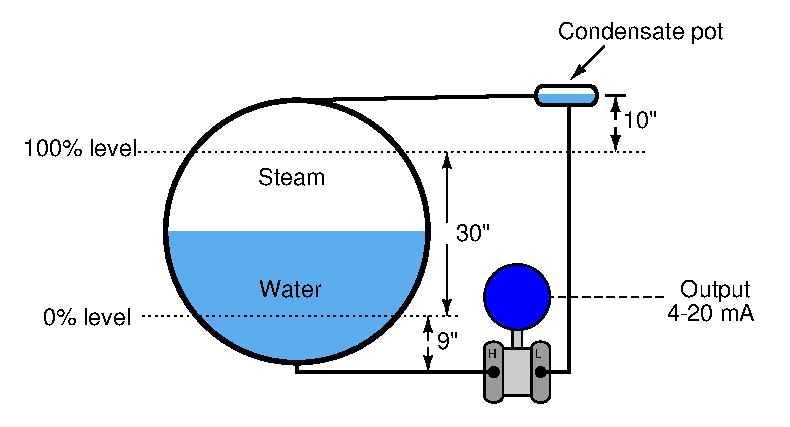
\includegraphics[width=15.5cm]{i00516x01.eps}$$

Anta en tetthet for (varmt) kjelvann på 36 lb/ft$^{3}$, en tetthet for damp i trommelen på 7 lb/ft$^{3}$, og en tetthet for (lunkent) vann i ``wet leg'' på 61.8 lb/ft$^{3}$. Hvis trykket på ``low'' (L)-siden av transmitteren er større enn trykket på ``high'' (H)-siden, skal differansetrykket oppgis som et negativt tall.

\vskip 10pt

\noindent
Poeng gis for korrekt beregning av hvert differansetrykk:

\begin{itemize}
\item{} {\bf (6 poeng)} Transmitter $\Delta$P ved 0\% vannivå = \underbar{\hskip 50pt} "W.C.
\item{} {\bf (6 poeng)} Transmitter $\Delta$P ved 50\% vannivå = \underbar{\hskip 50pt} "W.C.
\item{} {\bf (6 poeng)} Transmitter $\Delta$P ved 100\% vannivå = \underbar{\hskip 50pt} "W.C.
\end{itemize}

\underbar{file i00516}
%(END_QUESTION)





%(BEGIN_ANSWER)

\begin{itemize}
\item{} {\bf (6 poeng)} Transmitter $\Delta$P ved 0\% vannivå = \underbar{\bf -38.832} "W.C.
\item{} {\bf (6 poeng)} Transmitter $\Delta$P ved 50\% vannivå = \underbar{\bf -31.864} "W.C.
\item{} {\bf (6 poeng)} Transmitter $\Delta$P ved 100\% vannivå = \underbar{\bf -24.896} "W.C.
\end{itemize}

%(END_ANSWER)





%(BEGIN_NOTES)


%INDEX% Measurement, level: hydrostatic pressure (suppressed zero)

%(END_NOTES)

